\chapter{Unclear age pattern, requiring expert priors: premenstrual syndrome}
\label{applications-priors_knots_select}

Epidemiological data without clear age-patterns are a reoccurring
theme in the GBD 2010 study.  Unclear age-patterns make expert priors
essential in the modeling process.  However, such cases are very
sensitive to the choice of prior assumptions, as shown in the
following example of premenstrual syndrome (PMS) in Western Europe.

PMS is a common cyclic disorder that affects women of reproductive
years during the period between ovulation and the onset of menses.
More than $200$ behavioral, psychologic and physical symptoms have been
associated with PMS, the most common being irritability, tension,
depression, bloating, weight gain and food cravings.  There is no
known cause or consistent
treatment. \cite{dickerson_premenstrual_2003, singh_incidence_1998,
  goodale_alleviation_1990}

A meta-analysis of data from a systematic review on the descriptive
epidemiology of premenstrual syndrome yielded $74$ prevalence
data points, of which $18$ were from Western Europe.  As seen from Figure
\ref{fig:app-pms_data}, the data are noisy, with overlapping and
heterogeneous age groups that show no clear age pattern.

    \begin{figure}[h]
        \begin{center}
            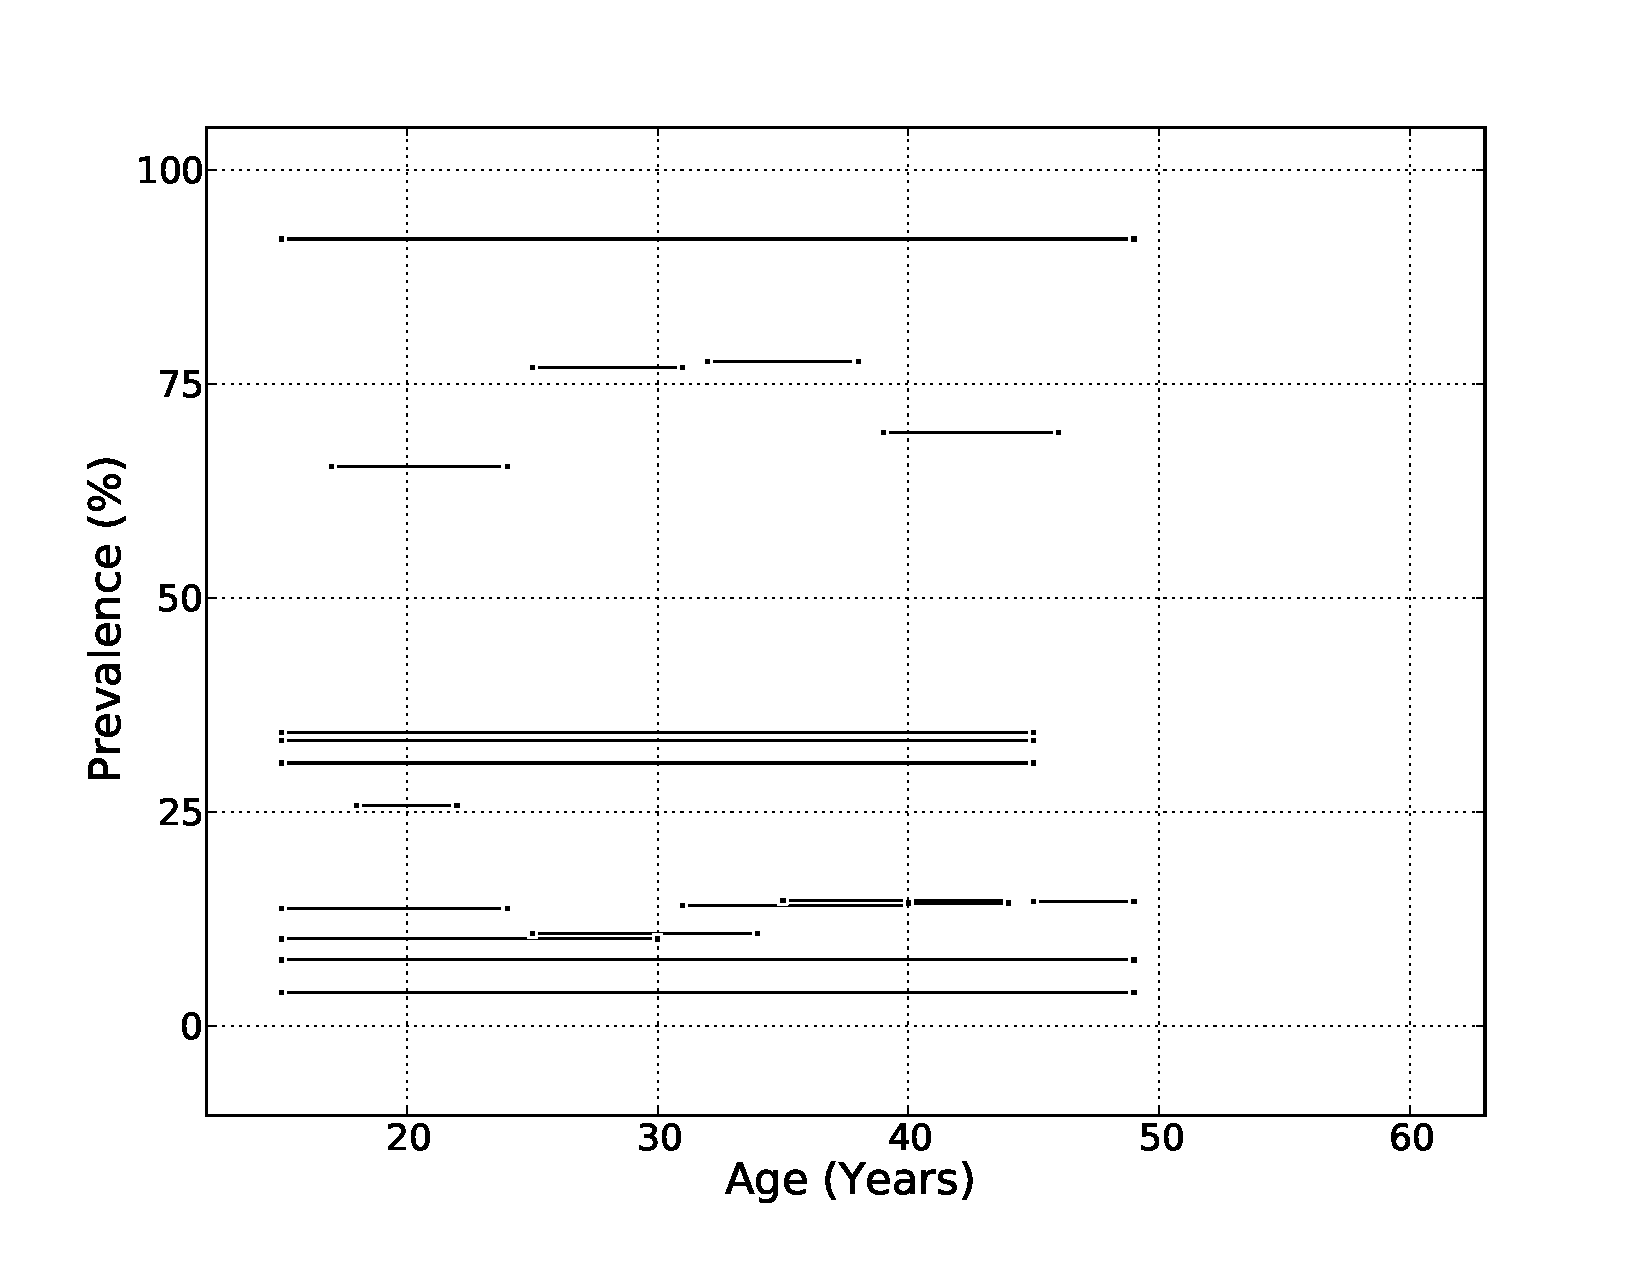
\includegraphics[width=\textwidth]{pms-data.pdf}
            \caption{Prevalence data for women with premenstrual
              syndrome in Western Europe.}
        \end{center}
        \label{fig:app-pms_data}
    \end{figure}

%% \section{Priors on level} \label{sec:app-priors on level}
In the absence of clear age patterns in the systematic review data
points, modeling decisions about knot location, age pattern levels,
and age pattern slopes have substantial influence on the estimates of
diseaes prevalence.  These decisions can also have unintended
consequences, as discussed in Chapter \ref{theory-age_pattern_model}.
To illustrate the effects, a sensitivity analysis including a variety 
of choices about knot location,
level values outside of the measured age intervals, and age pattern
slopes are compared and contrasted for estimating PMS prevalence.

As the prevalence data plotted in Figure \ref{fig:app-pms_data} show,
systematic review collected no data on population prevalence for women
younger than age 15 or older than age 50.  Since PMS is a disorder
related to the cycles of the female reproductive system, it is obvious
that the data outside this age range are not present for biological
reasons.  However, this is not part of the spline model unless the
modeler includes it.  If no priors are included to inform
estimates in the young and old, then they are extrapolated from the
levels where there is data, as seen in Figure
\ref{fig:app-pms prios_on_level}.  Here expert knowledge is needed to
inform the model that cases are not expected outside of the age range
where they have been measured.

    \begin{figure}
        \begin{center}
            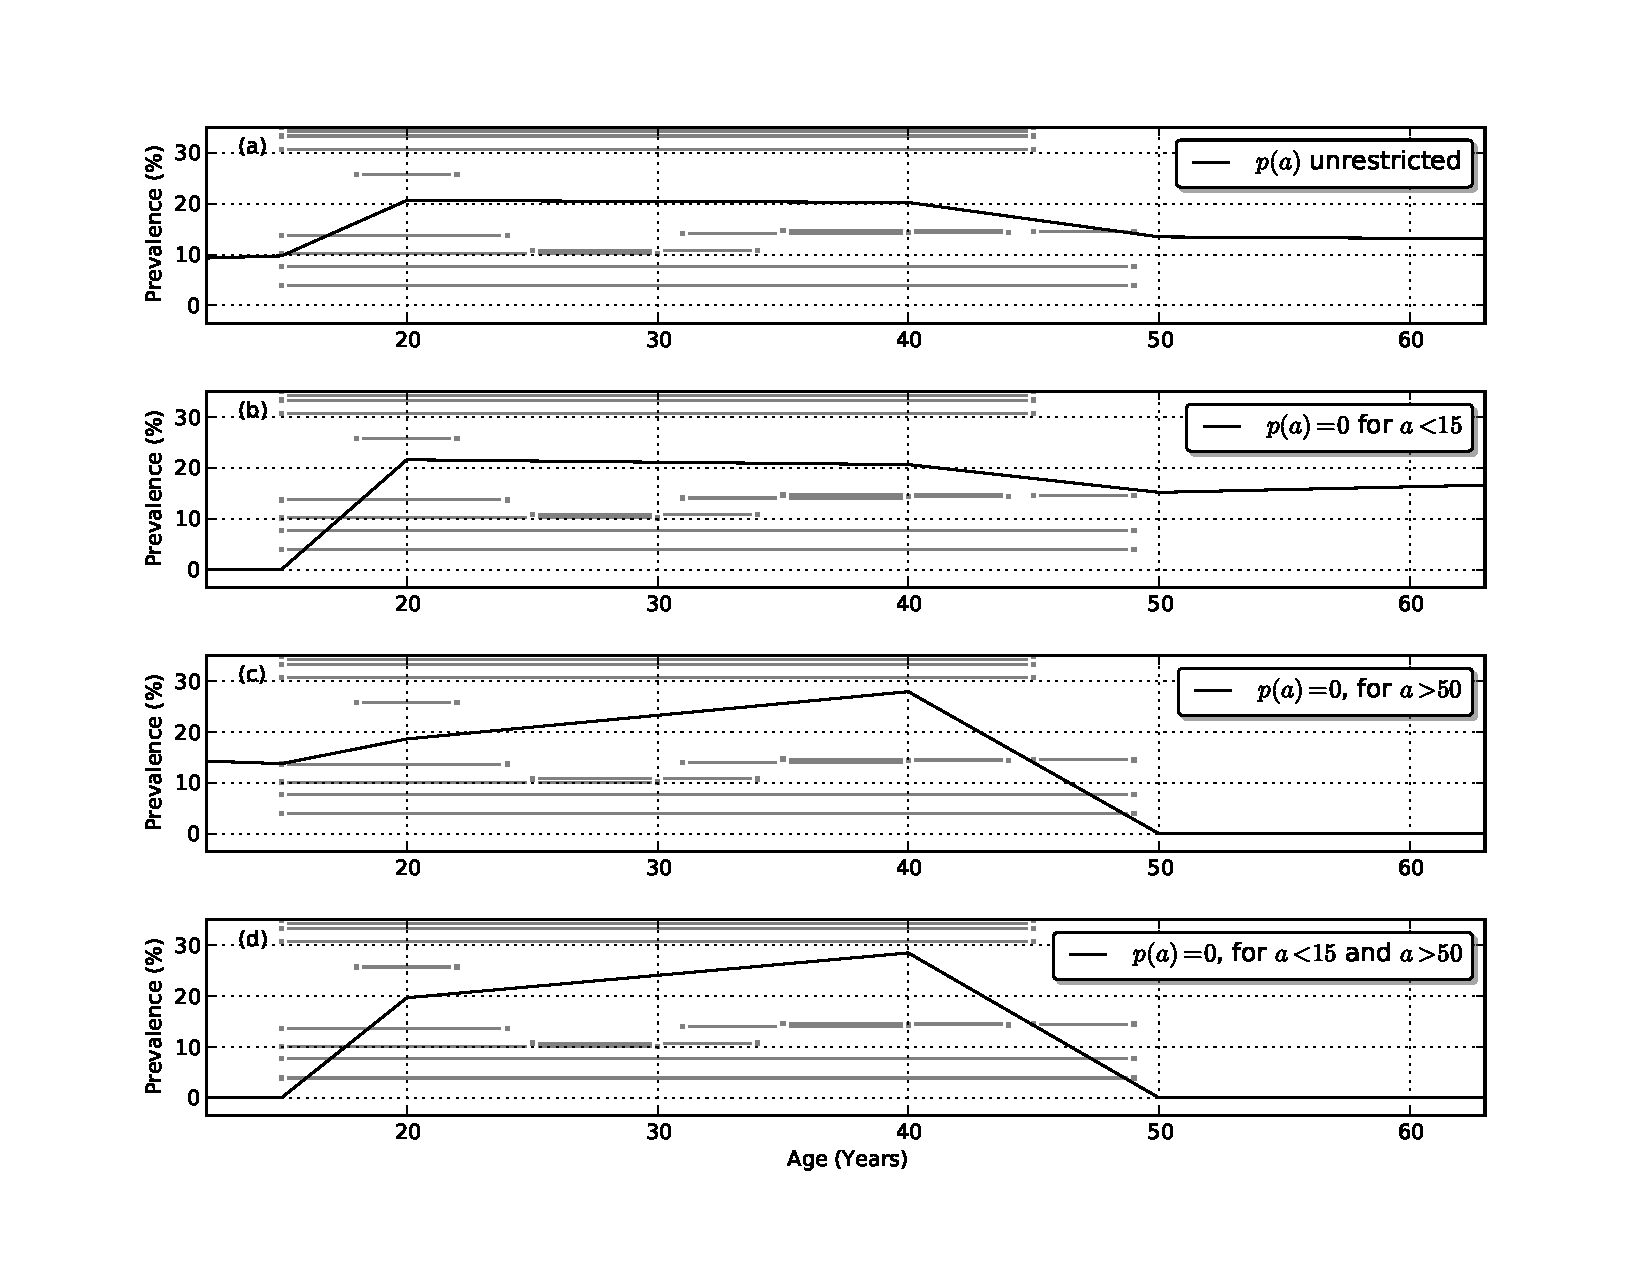
\includegraphics[width=\textwidth]{pms-priors.pdf}
        \end{center}
        \caption{PMS is a disorder related to the cycles of the female
          reproductive system for which systematic review revealed
          sparse and noisy data, shown here for Western Europe.  Panel
          (a) shows that without a level prior to inform the model
          that prevalence data is not present outside of the ages
          15-50 for biological reasons, it will create prevalence
          estimates for all ages, regardless of biological
          feasibility.  Restricting prevalence to zero changes the
          prevalence estimates substantially. Panel (b) shows the
          effect of assuming $p(a) = 0$ for $a<15$. Panel (c) shows
          the effect of assuming $p(a) = 0$ for $a>50$. Panel (d)
          shows the effect of assuming $p(a) = 0$ for $a<15$ and
          $a>50$.}
        \label{fig:app-pms prios_on_level}
    \end{figure}

%% \section{Knot location}
As previously discussed in Chapters
\ref{theory-age_group_model-overlapping_data} and
\ref{applications-splines_knot_loc}, age-specific hazards are modeled
with splines, using knots to partition the age range into intervals.
Models will not be very sensitive to choice of knots with ample data
and clear age patterns.  However, with sparse and noisy data without a
clear age pattern, the number and location of knots can influence the
model results substantially as seen in Figure \ref{fig:app-pms knot_loc}.
Choosing the number and location of knots a priori using expert
knowledge allows the user to determine critical features of the model.

    \begin{figure}
        \begin{center}
            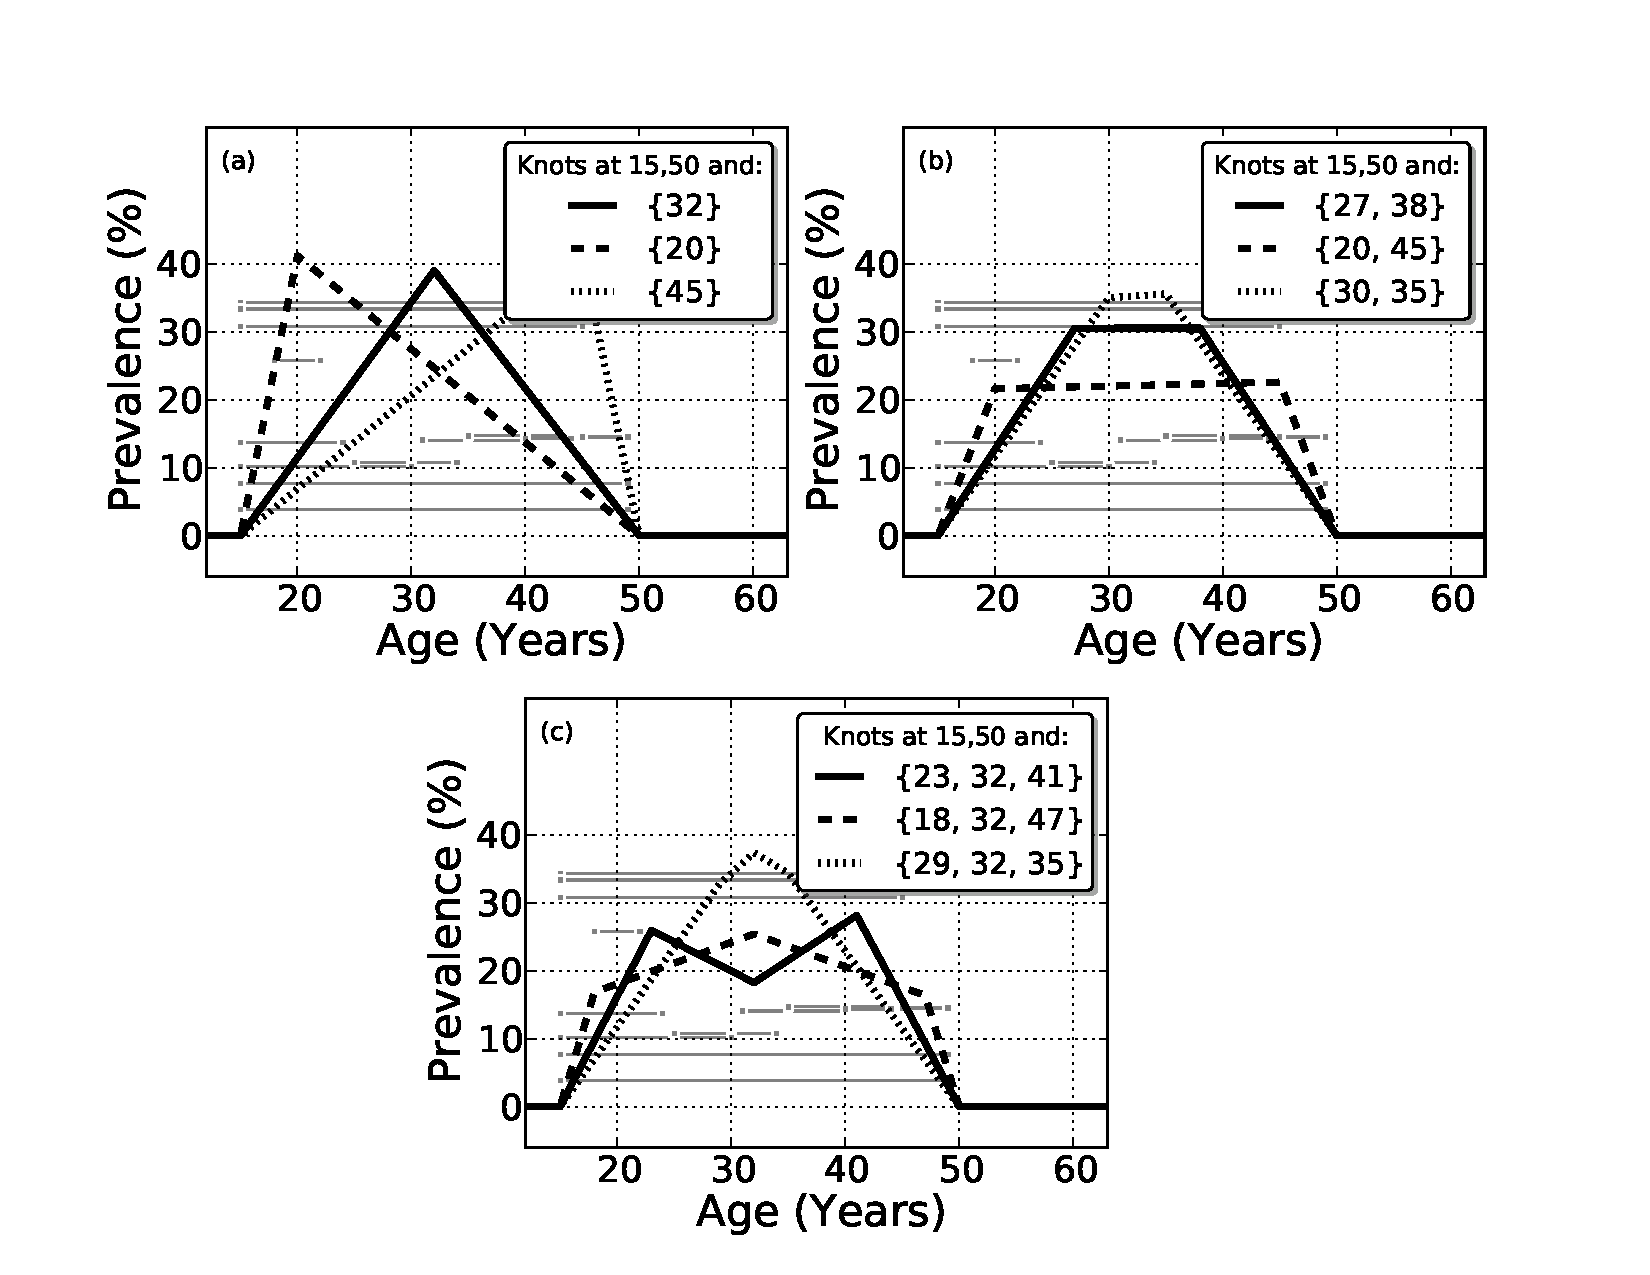
\includegraphics[width=\textwidth]{pms-knot_location.pdf}
        \end{center}
        \caption{All panels have knots at \{0, 15, 50, 100\} and vary
          the number and location of knots between the ages of 15 and
          50 to show the sensitivity of knot selection sparse and
          noisy data without a clear age pattern. Even with 1 knot,
          the placement at age 20, 32 or 45 gives markedly different
          estimates of PMS prevalence in Western Europe (panel (a)).
          Panel (b) uses 2 knots and varies their locations at \{27,
          38\}, \{20, 45\}, or \{30, 35\} while panel (c) uses 3 knots
          at locations \{23, 32, 41\}, \{18, 32, 47\} and \{29, 32,
          35\}.}
        \label{fig:app-pms knot_loc}
    \end{figure}

%% \section{Priors on monotonicity}
Another common prior for age patterns is the belief that the
epidemiologic parameter increases or decreases over a certain age
range.  As seen in Figure \ref{fig:app-pms dir}, priors on
monotonicity between the critical ages of 25 and 40 have a large
effect on the prevalence estimate for Western Europe.

    \begin{figure}
        \begin{center}
            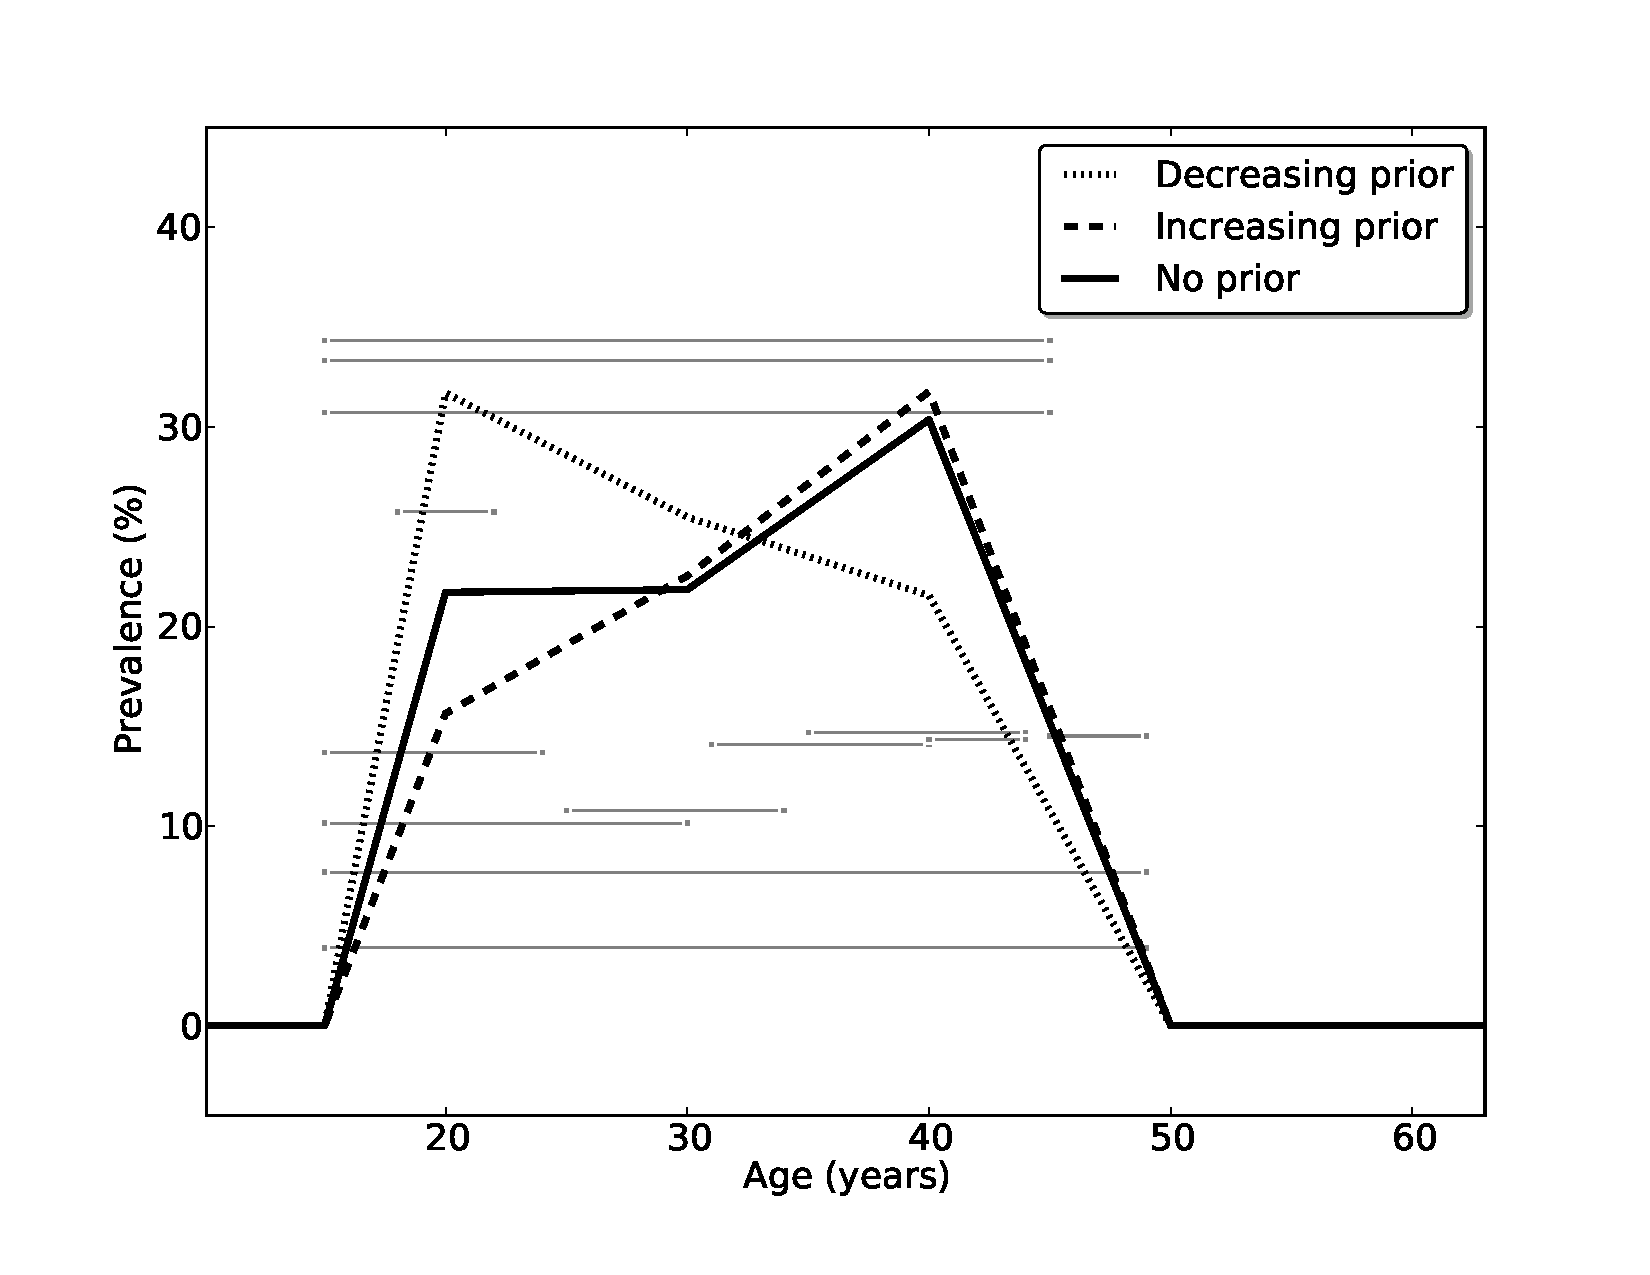
\includegraphics[width=\textwidth]{pms-direction.pdf}
        \end{center}
        \caption{Between the ages of 25-40, the prior on monotonicity
          makes a large impact on the prevalence estimates for women
          in Western Europe with premenstrual syndrome.}
        \label{fig:app-pms dir}
    \end{figure}

Knot selection, and priors on level and monotonicity play an important
role in the modeling process and in the sensitivity analysis.  However,
when the data is not sufficient to understand the age pattern, the
model compensates by producing a large uncertainty, as seen in
Figure \ref{fig:app-pms best}.  Figure \ref{fig:app-pms best} uses knots
at \{0, 15, 20, 30, 40, 50, 100\} and has no prior on monotonicity but
uses a prior on level to restrict the model to between ages 15-50.  This
example has identified an area of future research as PMS does not have enough
data to inform an age pattern--some studies say almost all women experience
it and some studies say none do.  In such cases, making the most informed
possible decisions (such as restricting the model to ages 15-50 for biological
reasons) and accepting a large uncertainty interval says the truth: we just don't know.

    \begin{figure}
        \begin{center}
            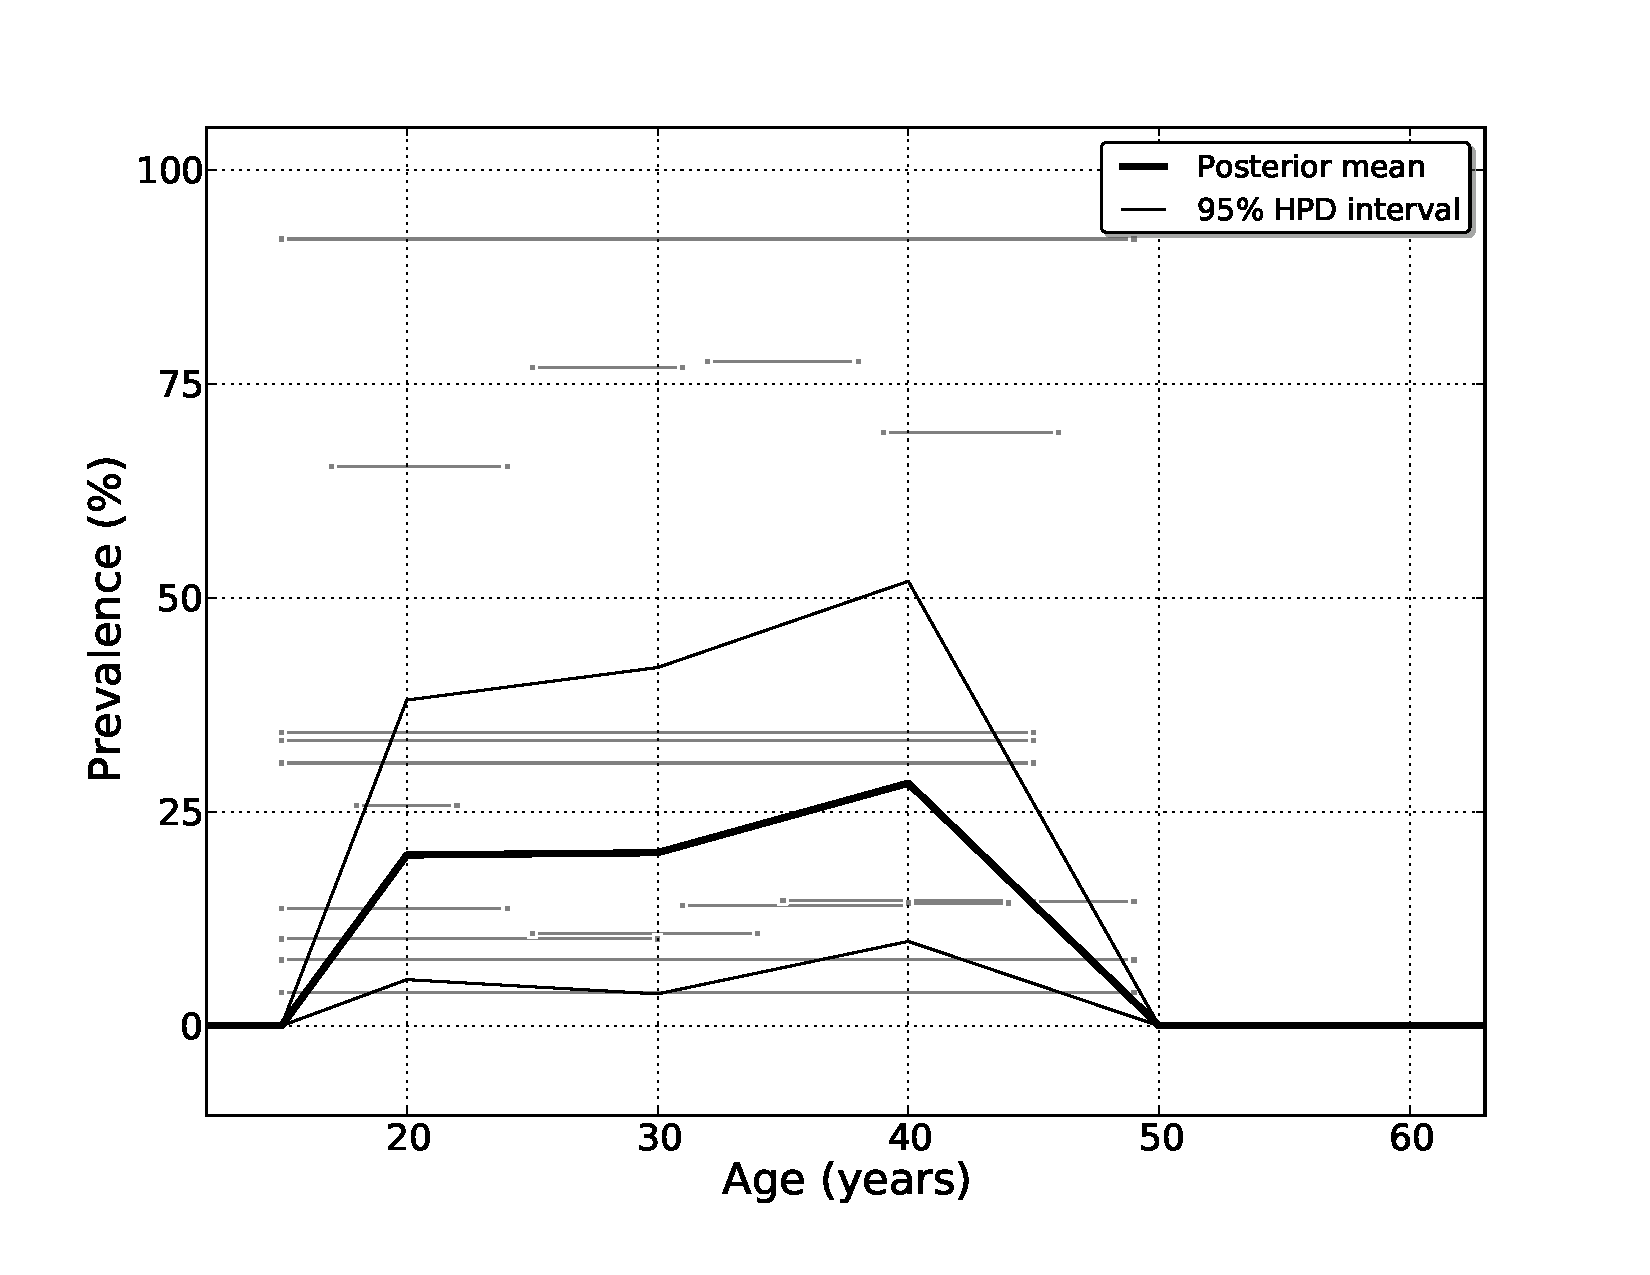
\includegraphics[width=\textwidth]{pms-best_model.pdf}
        \end{center}
        \caption{Prevalence estimates for women
          in Western Europe with premenstrual syndrome.}
        \label{fig:app-pms best}
    \end{figure}









